%%%%%%%%%%%%%%%%%%%%%%%%
%%%%Document Type   %%%%
%%%%%%%%%%%%%%%%%%%%%%%%

\documentclass[11pt]{article}

%%%%%%%%%%%%%%%%%%%%%%%%
%%%%Import Packages %%%%
%%%%%%%%%%%%%%%%%%%%%%%%

\usepackage{anysize}
\usepackage{minibox}
\usepackage{graphicx}
\usepackage{wrapfig}
\usepackage{xcolor}
\usepackage{listings}
\usepackage[font=small,labelfont=bf]{caption}
\usepackage{url}
\usepackage[T1]{fontenc}
\usepackage{subcaption}
\usepackage{amsmath}
\usepackage{bm}
\usepackage{booktabs}
\usepackage{multicol}
\hyphenchar\font=-1
\usepackage{titling}
\usepackage{enumitem}
\usepackage{multirow}
\usepackage{tabularx}
\usepackage{amssymb}
\usepackage{hyperref}
\usepackage{framed}
\usepackage{caption}
\usepackage{siunitx}
\usepackage{pgfplots}
\usepackage{circuitikz}
\usepackage{tikz}
\usetikzlibrary{shapes,arrows}
\usepackage[utf8]{inputenc}
\setcounter{secnumdepth}{5}
\setcounter{tocdepth}{5}


%%%%%%%%%%%%%%%%%%%%%%%%
%%%%Definitions     %%%%
%%%%%%%%%%%%%%%%%%%%%%%%

\newcommand{\mathbold}[1]{\boldsymbol{\mathrm{#1}}}
\newcommand{\mean}[1]{\langle #1 \rangle}
\newcommand{\leftright}[1]{\left( #1 \right)}

\tikzstyle{decision} = [diamond, draw, fill=blue!20, 
    text width=6em, text badly centered, node distance=3cm, inner sep=0pt]
\tikzstyle{block} = [rectangle, draw, fill=green!20, 
    text width=7em, text centered, rounded corners, minimum height=2em]
\tikzstyle{end} = [rectangle, draw, fill=red!20, 
    text width=7em, text centered, rounded corners, minimum height=2em]
\tikzstyle{line} = [draw, -latex']
\tikzstyle{cloud} = [draw, ellipse,fill=red!20, node distance=3cm,
    minimum height=2em]

%%%%%%%%%%%%%%%%%%%%%%%%
%%%%Title Info      %%%%
%%%%%%%%%%%%%%%%%%%%%%%%

\title{Thermodynamic simulations using the Ising model}
\author{Siddharth Amrat}
\date{December 2014}
\marginsize{1cm}{1cm}{1cm}{1cm}

%%%%%%%%%%%%%%%%%%%%%%%%
%%%%Document body   %%%%
%%%%%%%%%%%%%%%%%%%%%%%%

\begin{document}

\maketitle

\begin{abstract}
The Ising model is a simplified model of the spin-spin interactions between neighbouring atoms which gives rise to properties of the material such as specific heat capacity and magnetic susceptibility. The Metropolis algorithm is used to model the behaviour of a square array of atoms as the temperature changes. The phase transition was found to occur at a value of $\beta \approx 0.4$. In subsequent run throughs, the value of $\beta$ was held constant whilst the external magnetic field was varied.
\end{abstract}

\section*{Introduction}
A ferromagnet is a material which exhibits a net magnetic field in the absence of an external magnetic field. The Ising model is used to model the behaviour of ferromagnets and can be used to determine the behaviour near a phase transition.

The model is based on a microscopic view of the material. For this version of the model, we will be using a 2-D square array as show in Table~\ref{isingarray}.

\begin{table}[h]
\centering
\begin{tabular}{|l|l|l|l|l|}
\hline
$\uparrow$ & $\downarrow$ & $\downarrow$ & $\uparrow$ & $\downarrow$ \\ \hline
$\uparrow$ & $\downarrow$ & $\uparrow$ & $\downarrow$ & $\downarrow$ \\ \hline
$\downarrow$ & $\downarrow$ & $\downarrow$ & $\uparrow$ & $\downarrow$ \\ \hline
$\uparrow$ & $\downarrow$ & $\uparrow$ & $\downarrow$ & $\downarrow$ \\ \hline
$\downarrow$ & $\uparrow$ & $\downarrow$ & $\downarrow$ & $\uparrow$ \\ \hline
\end{tabular}
\caption{An example 5x5 array}
\label{isingarray}
\end{table}

Each atom is signified by a cell in the array and each cell has either spin-up ($+1$) or spin-down ($-1$). By considering these spins we can write expressions for the total interaction energy between the cells. This is given by:
\begin{equation} \label{eq:E}
E = -\frac{1}{2}\sum_{i, j}J_{ij}\mathbold{S}_{i}\cdot\mathbold{S}_{j} - \mu\sum_{k}\mathbold{S}_{k}\cdot\mathbold{B}
\end{equation}
where $J$ is the spin-spin interaction energy per spin squared and $\mu\mathbold{B}$ is the external magnetic field interaction energy per spin. The key point here are that when considering the spin-spin interactions, only the interactions between neighbouring sites are considered. So, for a central site, only the adjacent sites (up, down, left and right) contribute to the total energy and an assumption is made that the other sites do not \cite{kim}.

The aim of this project was to investigate the following quantities and how they vary as the algorithm is run:
\begin{multicols}{2}
\begin{itemize}
\item Total Energy (Equation~\ref{eq:E})
\item Magnetisation (Equation~\ref{eq:M})
\item Specific Heat Capacity (Equation~\ref{eq:C})
\item Magnetic Susceptibility (Equation~\ref{eq:Chi})
\end{itemize}
\end{multicols}

\section*{Method}
The Metropolis algorithm uses the Monte Carlo method of randomly sampling\cite{kingham}. The algorithm is shown in Figure~\ref{fig:flow}. Outside of the algorithm described in Figure~\ref{fig:flow}, there is another to check the state of the system and evaluate whether or not equilibrium has been reached. The metropolis algorithm is run initially for 20,000 iterations. During these iterations, the average energy of the last 2,500 iterations is taken and stored in a list. After the first 20,000 iterations, these averages are compared and if the value for the energy has not changed by a significant amount then the system is considered as being in equilibrium.

Once this state has been reached, the metropolis algorithm is run for another 10,000 and the measurements of $E$ and $S$ are taken from this and later used to calculate $C$ and $\chi$.

\begin{figure}[!ht]
\centering
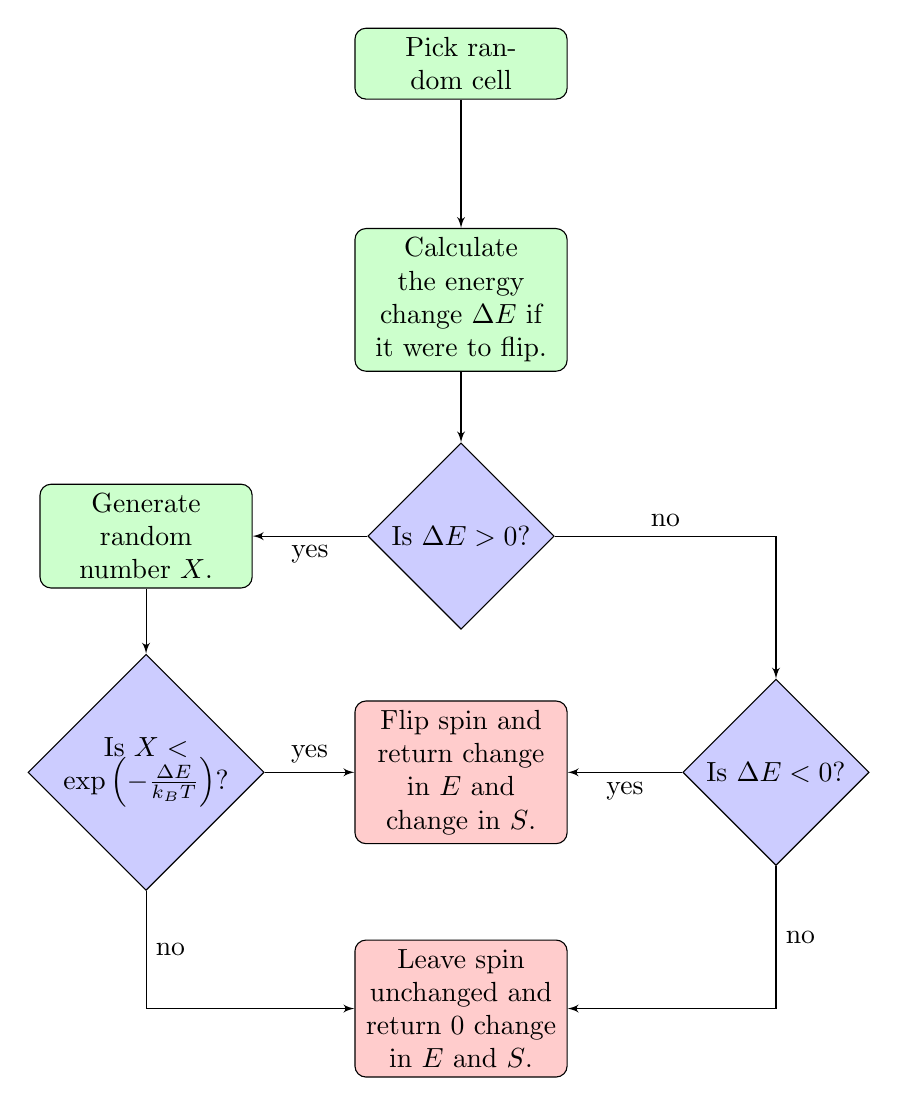
\begin{tikzpicture}[node distance = 2cm, auto]
    % Place nodes
    \node [block] (init) {Pick random cell};
    \node [block, below of=init, node distance=3cm] (deltaE) {Calculate the energy change $\Delta E$ if it were to flip.};
    \node [decision, below of=deltaE] (gt0) {Is $\Delta E > 0$?};
    \node [end, below of=gt0, node distance=3cm] (returnlt0) {Flip spin and return change in $E$ and change in $S$.};
    \node [decision, right of=returnlt0, node distance=4cm] (lt0) {Is $\Delta E < 0$?};
    \node [decision, left of=returnlt0, node distance=4cm] (metropolis) {Is $X < \mathrm{exp}\left(-\frac{\Delta E}{k_{B}T}\right)$?}; 
    \node [end, below of=returnlt0, node distance=3cm] (stop) {Leave spin unchanged and return $0$ change in $E$ and $S$.};
    \node [block, left of=gt0, node distance=4cm] (returngt0) {Generate random number $X$.};
    % Draw edges
    \path [line] (init)       -- (deltaE);
    \path [line] (deltaE)     -- (gt0);
    \path [line] (gt0)        -| node [near start] {no}(lt0);
    \path [line] (gt0)        -- node {yes} (returngt0);
    \path [line] (lt0)        -- node {yes} (returnlt0);
    \path [line] (returngt0)  -- (metropolis);
    \path [line] (lt0)        |- node [near start] {no}(stop);
    \path [line] (metropolis) -- node {yes} (returnlt0);
    \path [line] (metropolis) |- node [near start] {no} (stop);
\end{tikzpicture}
\caption{Flow chart describing the implementation of the metropolis algorithm.}
\label{fig:flow}
\end{figure}

Aside from the Metropolis algorithm, a few other processes were required. One was the calculation of the total energy of an array. Considering the first term in Equation~\ref{eq:E}, each site has four neighbours. However, if the sum of the four neighbours is taken then there would be some double counting and so to avoid this, a method called \texttt{neighbour\_energy} was written which only counted the contribution to the total energy from those neighbours which are to the right and below the current site. This ensures that iterating through the whole array (with periodic boundary conditions) gives the contribution of every pairwise interaction between the sites.

In the code the equations for energy, magnetisation, specific heat capacity and magnetic susceptibility are not used in their original form, but rather a substitution is made where $\beta = J/k_{B}T$. This means that the model can be investigated by only varying $\beta$ as opposed to both $J$ and $T$.

The program can be run in one of two modes. In one mode the external field is held constant (default value of 0) and the $\beta$ is increased from 0 to 1. In the other mode, the $\beta$ value is held constant while the external magnetic field is varied.

To improve the efficiency of the algorithm, the total energy was only calculated once at the start of the simulation. For every subsequent iteration, the energy would be updated by adding the change in energy caused by flipping (or not flipping) a site. In addition to this, once the system reached equilibrium for one value of $\beta$, the final state of the array and the energy would be fed back in with the total energy of that array, again saving time.

In the main function which calls this algorithm, the entire process starting from $\beta=0$ is repeated multiple times and averaged to give a more accurate representation.

Problems which arose in early implementations were \texttt{MemoryError}s which were caused by the storage of large lists in RAM. Generators were used for iterative methods so that this would no longer occur and allows much larger array sizes to be tested instead of just a small 10 x 10 array.

\section*{Results}
As mentioned before, the program could be run in one of two ways. Either the value of $\beta$ is varied or the external magnetic field strength is varied. In the case of varying $\beta$, the external magnetic field strength was set as $0$.

It was found that a phase transition occurs at a $\beta$ value of approximately 0.4. This can be seen in Figure~\ref{fig:changingbeta} which shows peaks in the specific heat capacity and magnetic suscepitibility graphs. Correspondingly, the graphs for energy and magnetic susceptibility also exhibit interesting behaviour at the same value of $\beta$.

\begin{figure}[!ht]
\centering
\includegraphics[width=\textwidth]{figure_4.png}
\caption{Graph against beta which goes from 0 to 1 in 100 steps. (*) The units in Figure C are units of J, that is the spin-spin coupling interaction between adjacent sites.}
\label{fig:changingbeta}
\end{figure}

In Figure~\ref{fig:changingbeta}D, it can be be seen that the magnetisation stays roughly level until $\beta$ reaches 0.4 at which point the material becomes magnetic as evidenced by the value of magnetisation levelling off at 1.

These graphs were acquired with an array size of 25 x 25. For smaller arrays, the results were more sporadic and for larger arrays, a prohibitively large number of measurements would have had to been taken to investigate the behaviour at the phase transitions.

The other mode of operation was to hold $\beta$ constant and vary the external magnetic field. The graph of this behaviour can be seen in Figure~\ref{fig:changingfield}. This graph produces an expected result, which is that in the presence of an external magnetic field, the ferromagnet will align itself with that field when it reaches equilibrium as that is the lowest energy state. Also, from the graph of the energy it can be seen that the states are more stable the larger the magnitude of the external field.

\begin{figure}[!ht]
\centering
\includegraphics[width=\textwidth]{figure_2.png}
\caption{Graph showing how the total energy and magnetisation of the array changes as the external magnetic field is applied.}
\label{fig:changingfield}
\end{figure}

Further to this, the presence of an external magnetic field was studied in the case where $\beta$ was varied. It is expected that with the presence of the magnetic field, the ferromagnet would have a preferred overall spin which aligns with the external field. The results can be seen in Figures~\ref{fig:energyfieldchange} and~\ref{fig:magnetisationfieldchange}.

\begin{figure}[!ht]
\centering
\begin{subfigure}[b]{0.49\textwidth}
\includegraphics[width=\textwidth]{elecfields.png}
\caption{Energy against $\beta$.}
\label{fig:energyfieldchange}
\end{subfigure}
\begin{subfigure}[b]{0.49\textwidth}
\includegraphics[width=\textwidth]{magfield.png}
\caption{Magnetisation against $\beta$.}
\label{fig:magnetisationfieldchange}
\end{subfigure}
\caption{The graphs here show the differences in the energy and magnetisation of the lattice for different strengths of external magnetic field. The number in the legend corresponds to the value of $\mu \mathbold{B}$ in terms of $J$.}
\label{fig:multiplefield}
\end{figure}

\section*{Discussion}
The results bring up many interesting phenomena, particularly the phase transition. Firstly the individual situations will be discussed.

\subsection*{Varying $\beta$}
In the first scenario, the external magnetic field is held constant at $\mathbold{B}=0$ and starting from 0, the system is propagated until equilibrium is reached. After this point, measurements and taken and then the value of $\beta$ is incremented. As seen in Figure~\ref{fig:changingbeta}, there is a peak in the region of $\beta=0.4$ in both the specific heat capacity and the magnetic susceptibility graphs.

These peaks correspond to the phase transition of a ferromagnet at which point there is a marked increase in the quantities. This sudden behaviour is also noticed in the graphs of energy and magnetisation. When going along the $\beta$ axis from 100 to 0, the energy stays roughly constant until it reaches the phase transition at which point the energy increases, which implies that the region is less favourable.

This is reiterated by the fact that in the region of $\beta>0.4$, Figure~\ref{fig:changingbeta}D is a flat line at 1.0 which means that the array is magnetised. This explains the energy being flat as well. As the array is fully magnetised, the spins are aligned and the total energy of the array is minimised. Note that the magnetisation is not always 1.0, but rather $\pm\;1.0$ due to the fact that the spins in the array could either be lined up all with negative spin or all with positive spin.

The reason for the peak in the specific heat capacity and the magnetic susceptibility is due to the correlation length of the system approaching infinity. To understand this, consider an array in which all of the spins are randomly aligned. As $\beta$ is decreased, clusters start to form. These clusters are regions in which all the atoms are aligned with each other. The correlation length of the system relates to the size of these clusters\cite{kim}.

Clusters are energetically favourable structures due to the fact that all the spins are aligned. Eventually there will come a point where a single cluster spans the entire length of the array, at which point the correlation length becomes infinite. This is the phase transition of the system. In the case of $\beta$ being lowered, this corresponds to the ferromagnet spontaneously becoming magnetic. However, this also works in the opposite direction. As $\beta$ is increased, the originally magnetic ferromagnet loses its magnetisation at a certain point.

The specific heat capacity and magnetic susceptibility are both relate to the correlation length and that explains why the sharp peak appears at $\beta \approx 0.4$.

\subsection*{Varying $\mathbold{B}$}
For this test, shown in Figure~\ref{fig:changingfield}, a constant value of $\beta$ was used and $\mu \mathbold{B}$ was varied between $-J$ and $+J$. As would be predicted, the presence of an external magnetic field encourages the ferromagnet to reach equilibrium in a state which aligns with the field, so as to decrease the total energy of the system.

So it can be seen trivially that for $\mu \mathbold{B}\neq 0$ (100 on the graph's x-axis) that the magnetisation is firmly in the direction of the external field. There is a slight exception to this however. For small values of $\mu \mathbold{B}$,the overall magnetisation tends to alternate between -1 and 1. This is due to the random arrays generated. In some cases, the external field could be negative but the array has enough positive spin particles to allow for an overall positive magnetisation. However, this is only the case for small external fields and quickly dissipates.

The reason for this can be seen in the graph of energy in Figure~\ref{fig:changingfield}. The most stable configurations occur for the largest external magnetic fields of course, but near the center where $\mu \mathbold{B}$ is small, the graph of energy is flatter and so there is some small area in which a positive magnetisation can be had in an array with the presence of a negative external field.

\subsection*{Effect of changing external field on $E$ and $M$}
Figure~\ref{fig:multiplefield} shows graphs of energy and magnetisation with all of the same conditions except for the strength of the external magnetic field. It can clearly be seen that in the presence of a magnetic field, the system assumes a lower energy state due to the decreased energy associated with the second term from Equation~\ref{eq:E}.

Similarly, Figure~\ref{fig:magnetisationfieldchange} clearly shows that the greater the strength of the magnetic field, the faster the system will be fully magnetised.

Although these, are expected results, it is interesting to note that for the emergy, there appears to be a uniform linear relationship governing the final energy of the system which is evidenced by the uniform flat lines beyond 30 on the graph ($\beta>0.6$).

\subsection*{Implementation}
Although the algorithm is very simple, a big hindrance in this investigation was computing power. In reaching equilibrium for one value of $\beta$, the metropolis algorithm will be called in the order of $10^{6}-10^{7}$ times which, when combined with the fact that anywhere from 50-100 different $\beta$ values are used leads to a fairly slow program.

The program was run using Python, and although it is nominally an interpreted language, the core functions were split between modules to allow for precompiled bytecode to speed up processing. In addition to this, third party libraries were used for things such as calculating the value of the magnetic susceptibility from a large list of numbers. For example, the \texttt{statistics} module has an underlying codebase written in C to improve performance.

Some consideration was made into parallel programming but due to incompatability issues this was abandoned. A similar reason also explains the primitive nature of the \texttt{animation} module. The original plan was to create a video of the array over the whole process but storing all that information would require more RAM than is typically available on computers.
 
\section*{Conclusion}
In conclusion, the Ising model is the simplest model of a ferromagnet which can describe the macroscopic properties of specific heat capacity and magnetic susceptibility by using a microscopic model. It also successfully captures the phase transition and can be used to study the behaviour of the system at the point in more detail.

It was found that a phase transition for a 25 x 25 array occurs at a value of $\beta$ of approximately 0.4. This phase transition is the same for any starting array, be it random of ordered.

Upon further investigation, it was also found that the external magnetic field has a significant effect on the system and the overall energy of the system. In the absense of an external magnetic field, there is no preference either way to a ferromagnet being overall spin-up or spin-down, but once a ferromagnet is present, the favoured direction is to align with the direction of the field.

The scale of the experiment was limited by computing power. With larger arrays, more accurate and realistic simulations are possible, but in addition to greater accuracy there is also greater processing time required. In addition to this, the number of steps taken to get from $\beta=0$ to $\beta=1$ plays a big role. The larger the number of steps, the more accurately the phase transition can be studied but for each step added the execution time increases.

Parallel processing was a possibility but having tested a parallel programming solution on a college computer and seeing that it would not work this was abandoned. Given more time, some interesting areas would be to analyse the cluster sizes within the array and plot the characteristic size for each value of $\beta$.

\bibliographystyle{plain}
\bibliography{bib1}

\section*{Appendix}
\subsection*{Magnetisation}
\begin{equation} \label{eq:M}
\mathbold{M} = N^{-2}\sum_{k}\mathbold{S}_{k}
\end{equation}
\subsection*{Specific Heat Capacity}
\begin{equation}\label{eq:C}
C = N^{-2}\frac{1}{k_{B}T^{2}}\left(\langle E^{2}\rangle - \langle E\rangle ^{2}\right)
\end{equation}
\subsection*{Magnetic Susceptibility}
\begin{equation}\label{eq:Chi}
\chi = N^{-2}\frac{J}{k_{B}T}\left(\langle S^{2}\rangle - \langle S \rangle ^{2}\right)
\end{equation}
\subsection*{Equations as used in the program}
In the code, the constants $k_{B}$, $T$ and $J$ were not used. Instead, a substitution was made where $\beta = J/k_{B}T$.
\subsubsection*{Total Energy}
\begin{equation}\label{eq:normE}
E = -\frac{1}{2}\sum_{i, j}\mathbold{S}_{i}\cdot\mathbold{S}_{j} - \frac{\mu |\mathbold{B}|}{J}\sum_{k}\mathbold{S}_{k}\mathbold{\hat{B}}
\end{equation}
Here, the energy is given in units of $J$ (note, not Joules).
\subsubsection*{Specific Heat Capacity}
\begin{equation}\label{eq:normC}
C = N^{-2}\;k_{B}\;\beta^{2} \leftright{\mean{E^{2}} - \mean{E}^{2}}
\end{equation}
\subsubsection*{Magnetic Susceptibility}
\begin{equation}\label{eq:normChi}
\chi = N^{-2}\;\beta \leftright{\mean{S^{2}} - \mean{S}^{2}}
\end{equation}

\noindent\makebox[\linewidth]{\rule{\textwidth}{0.4pt}}

Word Count (excluding captions, appendices and headers) (as calculated by the \texttt{TeXcount} package for \LaTeX ): 2309
\end{document}